% Chapter 2

\chapter{Database and data structure} % Main chapter title

\label{Chapter5} % For referencing the chapter elsewhere, use \ref{Chapter1} 

\lhead{Chapter 5. \emph{Database and data structure}} % This is for the header on each page - perhaps a shortened title

%----------------------------------------------------------------------------------------

\section{Database}
As described, our data consists of two parts. \textit{Static} map data and \textit{dynamic} points of interests data. For the beginning, we were deciding between using relational database and XML based database. With each of them having some benefits, we took the following facts intro account during the consideration:
\begin{itemize}
\item Most of the data is static - information about the roads in Le Creusot will not change;
\item Dynamic data will rarely change - user will not often update information about the points of interest;
\item Relatively small amount of data - Le Creusot is a small city, so there is not a lot of information about the roads. This gives us the opportunity to read all the information to memory at the beginning, reducing the latency caused by queries to the database;
\item Easiness of install and mobility -  using relational database, requires installation of different software (SQL server, connectors, etc.) on the clients computer, which we wanted to avoid. 
\end{itemize} 
In the end we decided to use \textbf{XML based database}. We kept the two parts of the data split into separate XML files. We kept the OpenStreetMap data in the OSM file and created another XML file for POI data. This way, we could easily change either part of the data without compromising the other.
\subsection{Disadvantage}
Using XML based database has one big disadvantage, which we have to take into account. XML based database is saved into a file. This does not provide the ability to easily update POI data. Unfortunately, every time we update this data, we have to rewrite the whole file. This can in some occasions be the source of problems, as the writing to the file can be disrupted or cancelled, making the file unusable. However, we do not anticipate the user to update the data frequently, so we took this compromise.

\section{Data structure}
We have designed out class structure with the A* search algorithm and OpenStreetMap (OSM) file structure in mind. We followed the OSM structure, having a basic class called \textbf{Node}. In figure \ref{fig:types_db} we show the different types of classes we use with a small graphic representation for better understanding.
\begin{figure}[h]
\centering
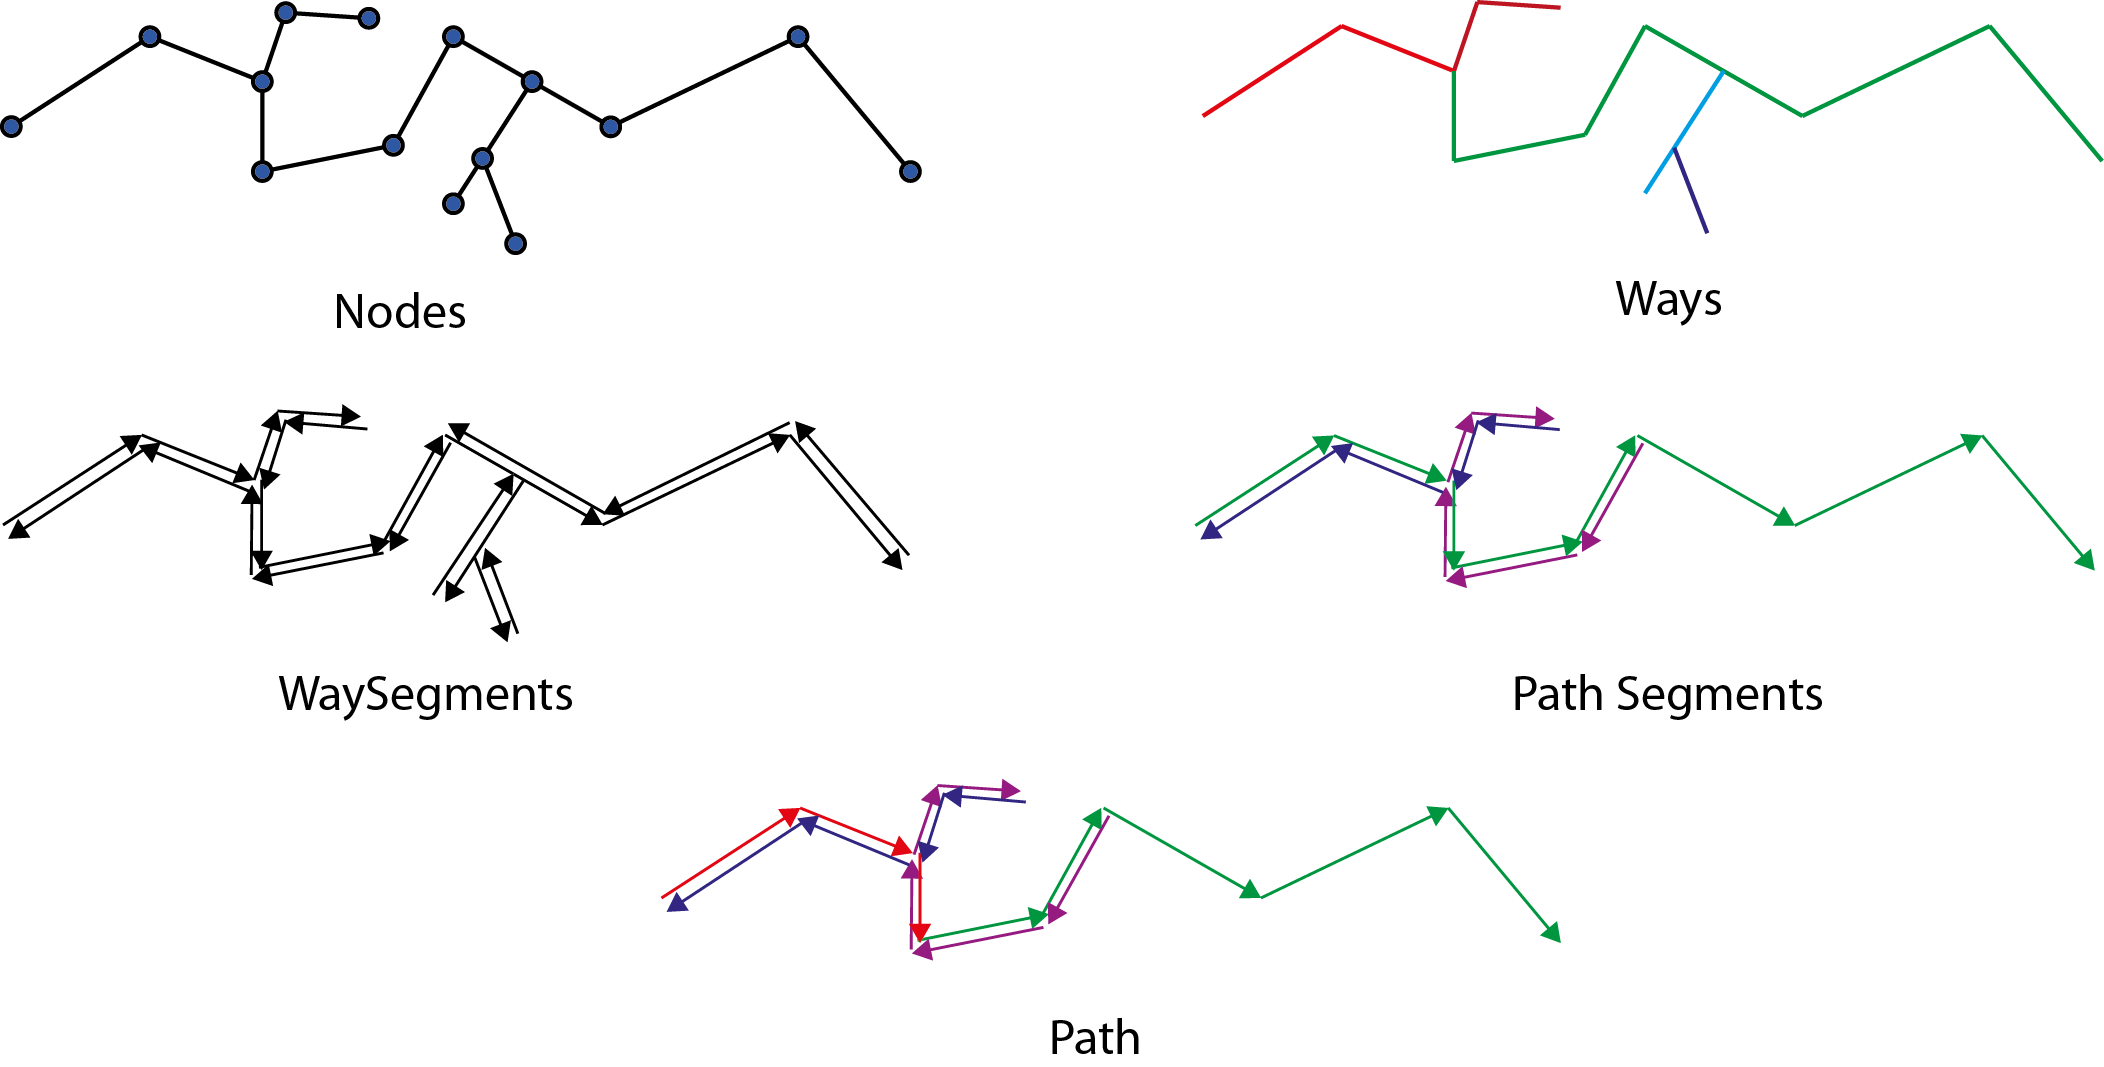
\includegraphics[width=0.8\linewidth]{../pictures/ways.png}
\caption{Different objects in our data structure}
\label{fig:types_db}
\end{figure}
\subsubsection{Node class}
It is used to represent a single point on the map. This can either mark a point of interest (POI), or can be a part of a Relation such as \textit{WaySegment, Building or Way}. It contains location information, some A* algorithm informations (weights, visited flags, etc.) and a vector of pointers of WaySegments to which we can traverse from this Node. This is important especially for A* algorithm, as it significantly reduce the time needed to find all possible and subsequently the correct next move.

\subsubsection{Way class}
Class implemented as in OSM file, to store the properties of each of the ways. It us usually used to represent whole streets, or part of the street that have the same properties. Each way is assigned a type (primary, secondary, etc.), direction (one-way, bidirectional) and access privileges (private or public).

\subsubsection{Relation class}
Relation is a base class from which we extend different relation classes (WaySegment, Building). It only contains a vector of pointers to Nodes that are in one specific relation and type of the relation.

\subsubsection{WaySegment class}
WaySegment is the main class for our path algorithms. WaySegment connects two nodes in a specific direction. This means that if the road between two nodes is bidirectional, we will create two WaySegment objects, one for each direction. We also have a pointer to an object Way, which belongs to the road traversing. This gives us the option of getting information about the road at any time.

\subsubsection{Building class}
Is a simple class containing all the nodes representing one building.

\subsubsection{PathSegment class}
It is a class that is used to store the result of a \textit{shortest path search}. It contains all the pointers to WaySegment objects we need to traverse in order to get from point A to B. 

\subsubsection{Path class}
Object that contains vector of PathSegment pointers. Path is the end result of any search. If the search is solely path from point A to B, the path is going to have only one PathSegment pointer. On the other hand, if we search for itinerary, Path will include multiple PathSegments, one for each pair of middle points.

\subsubsection{Database class}

Database is an main class for the whole database. It contains functions for correct parsing of XML files and also has containers \textit{(std::map)} with pointers to each of the classes created (Node,Way,Bulding,WaySegment). We use this to quickly retrieve the classes based on their ID, and to be sure to delete all created objects in the destructor of the class. We also used a boost implementation of a \textit{rtree} data structure to hold all the WaySegment objects to be able quickly do a spatial filtering. This is very useful in implementation of finding the close WaySegments.
\par
In figure \ref{fig:db_class} we can see the whole class diagram of the database part of the application in C++.
 \begin{figure}[h]
 \centering
 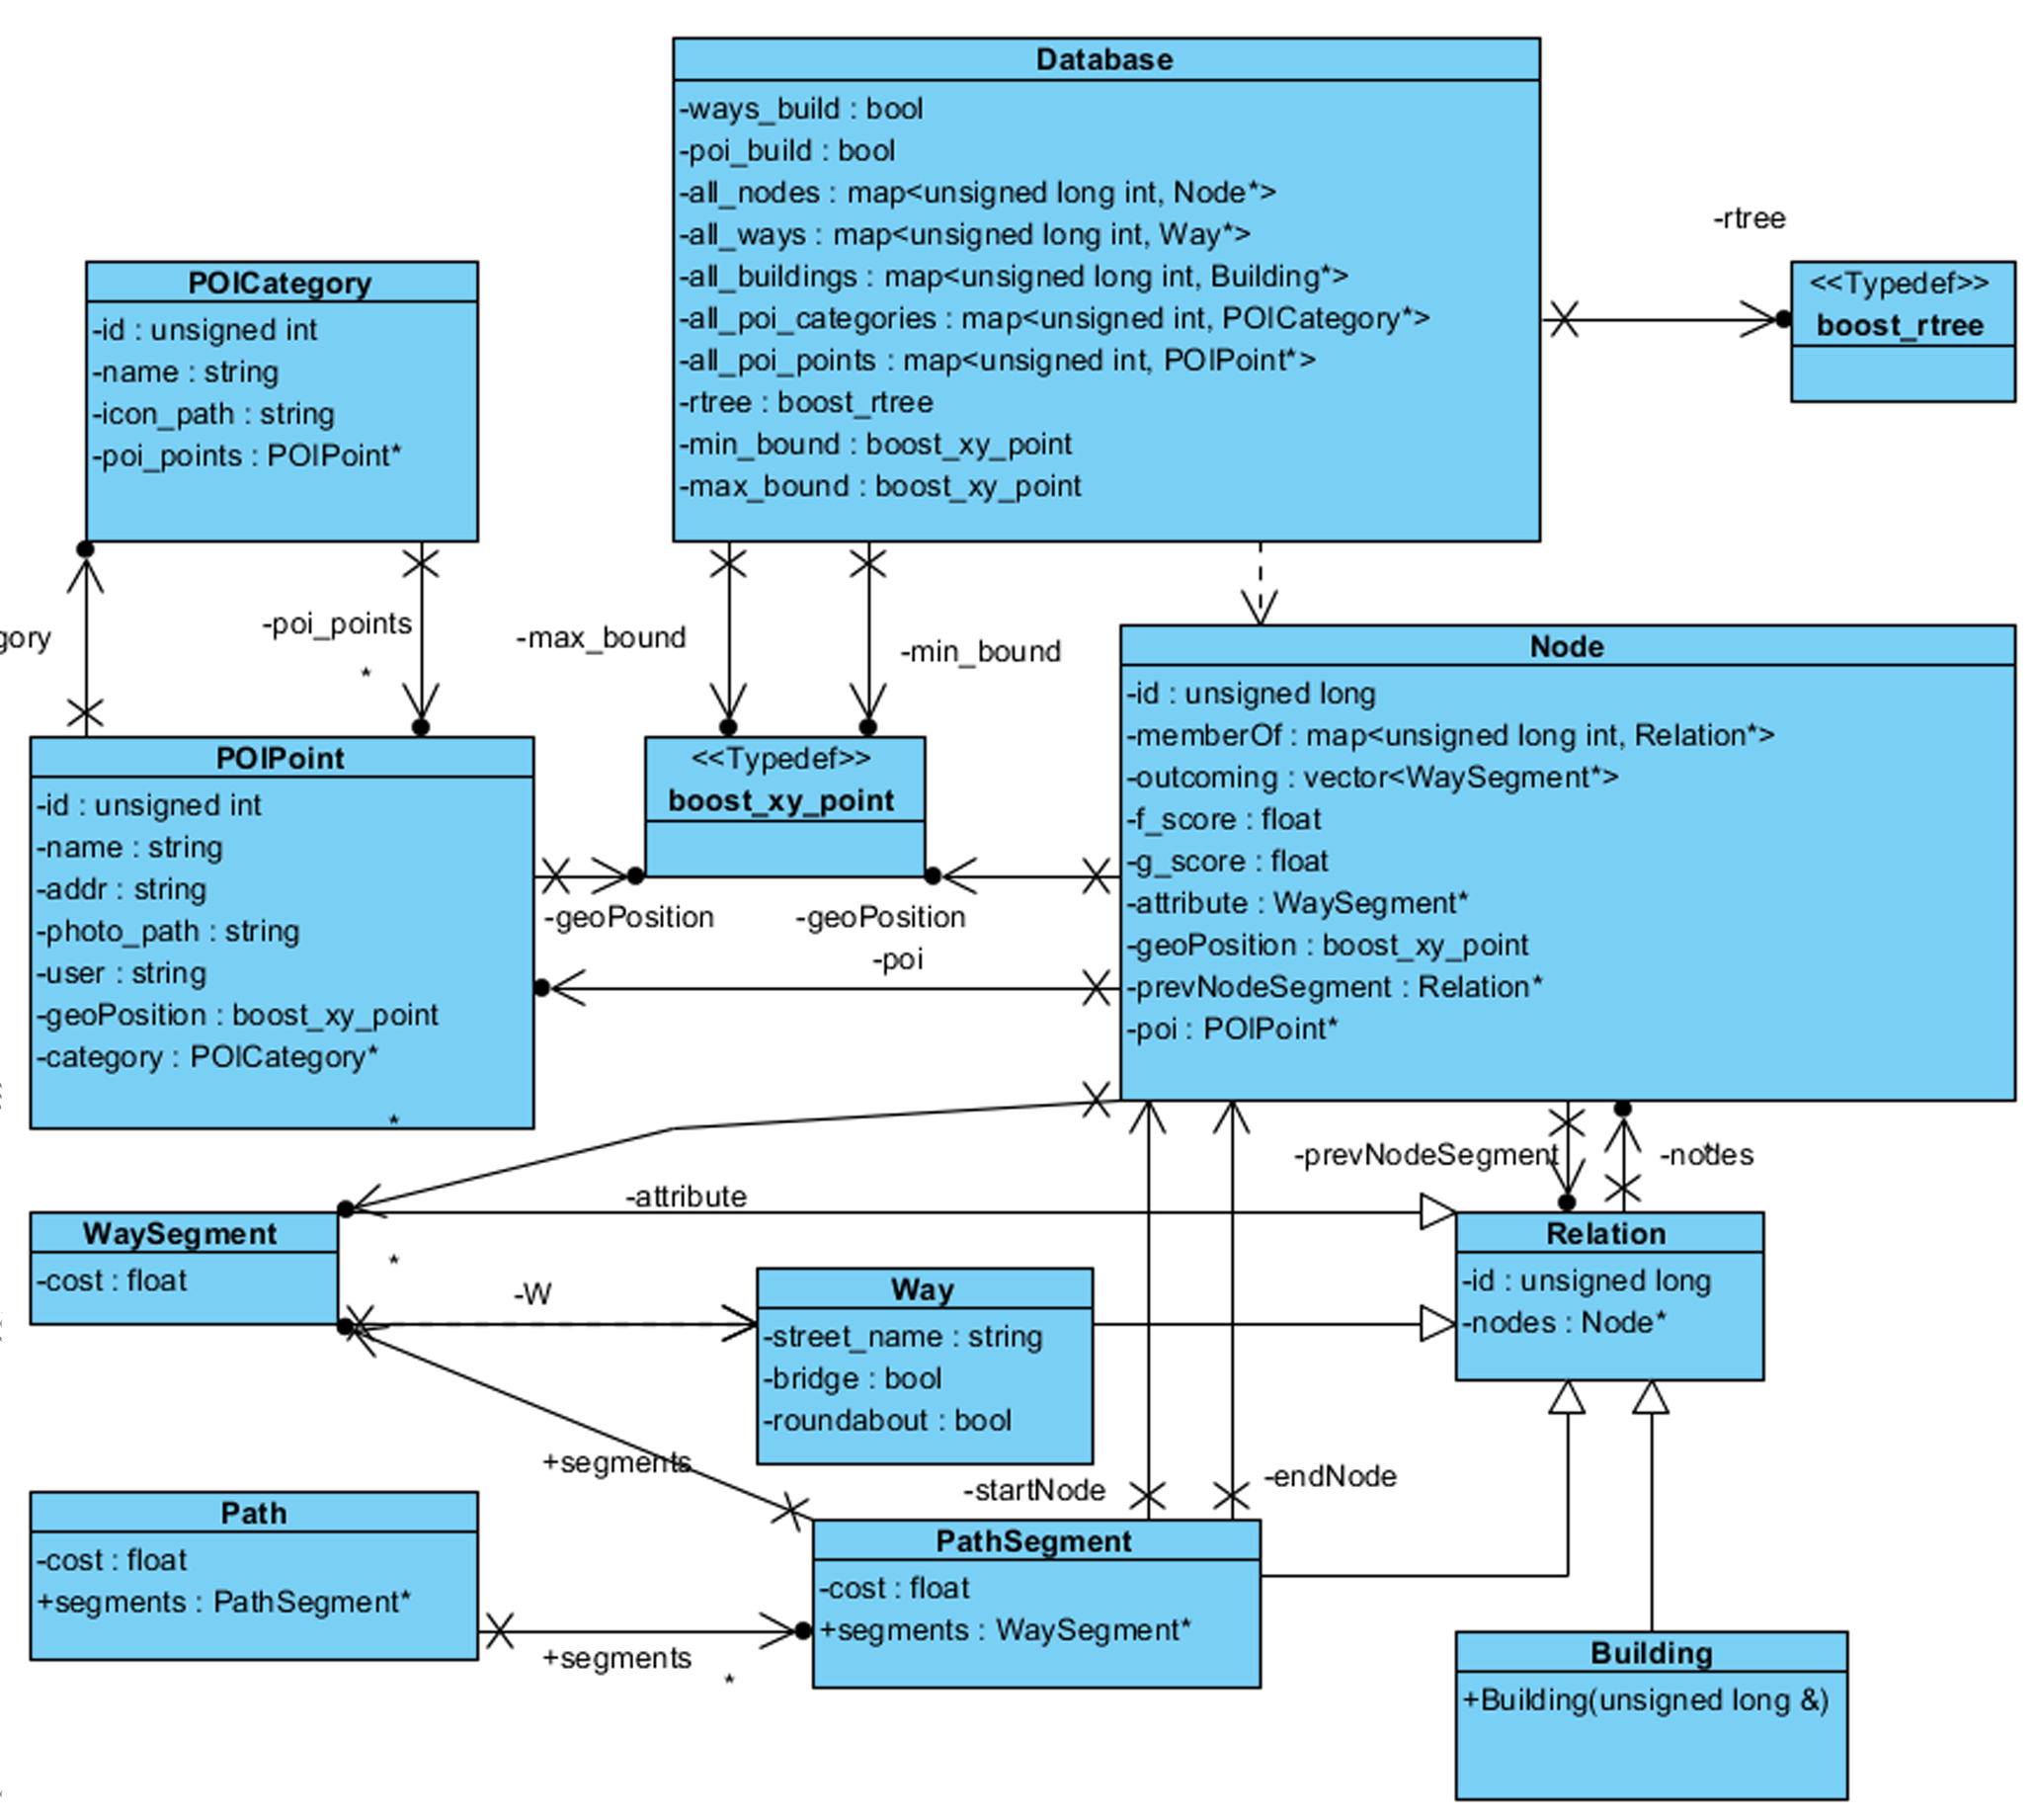
\includegraphics[width=0.9\linewidth]{../pictures/Class_Diagram.png}
 \caption{Class diagram}
 \label{fig:db_class}
 \end{figure}

